\documentclass{article}
\usepackage{graphicx}
\usepackage[letterpaper, total={6.5in, 9in}]{geometry}
\usepackage{listings}

\usepackage{xcolor}

\definecolor{codegreen}{rgb}{0,0.6,0}
\definecolor{codegray}{rgb}{0.5,0.5,0.5}
\definecolor{codepurple}{rgb}{0.58,0,0.82}
\definecolor{backcolour}{rgb}{0.95,0.95,0.92}

\lstdefinestyle{mystyle}{
    backgroundcolor=\color{backcolour},   
    commentstyle=\color{codegreen},
    keywordstyle=\color{magenta},
    numberstyle=\tiny\color{codegray},
    stringstyle=\color{codepurple},
    basicstyle=\ttfamily\footnotesize,
    breakatwhitespace=false,         
    breaklines=true,                 
    captionpos=b,                    
    keepspaces=true,                 
    numbers=left,                    
    numbersep=5pt,                  
    showspaces=false,                
    showstringspaces=false,
    showtabs=false,                  
    tabsize=4
}

\lstset{style=mystyle}

\title{Project 3: 7 Segment Display Counter Solution}

\author{Braidan Duffy\thanks{B.S. Ocean Engineering 2021\\M.S. Ocean Engineering 2023}}

\date{September 4, 2022}

\begin{document}

\maketitle

\section*{Undergraduate Students}
    \subsection*{Overview}
    This project is intended to demonstrate to students how to drive multiple LEDs using a multiplexed shift register, write data to a display module, and extend the work demonstrated in Project 2 by requiring button inputs to be held for certain actions to be performed.

    Undergraduate students will be considered to have completed the project when they demonstrate the following tasks:

    \begin{enumerate}
        \item Wire a button to an interrupt-capable input pin on the Arduino
            \subitem The button resets the counter when pressed
        \item Sound a buzzer whenever the reset is triggered
        \item Display the current counter value on a four-digit seven segment display driven by a shift register
        \item Make a "neat" breadboard where wires are easy to track, components are visible, cross-jumps are minimized, and wire colors are somewhat sensible (e.g. all orange for shift register driver pins, white for digit selectors, etc.)
    \end{enumerate}

    \subsection*{Grading}
    \begin{tabular}{ | p{1in} | p{1.75in} | p{1.75in} | p{1.75in} | }
        \hline
        \textbf{Category} & \textbf{No Credit} & \textbf{Half Credit} & \textbf{Full Credit} \\

        \hline
        Efficacy (70 pts) & 
        Student did not demonstrate their working project & 
        student demonstrated a working project, but it did not meet all of the requirements specified in the project handout & 
        student demonstrated a feature-complete project that accomplished all of the goals specified in the project handout \\
        \hline
        Breadboard neatness (10 pts) & 
        Student did not show a breadboard, or it is exceptionally difficult to trace wires or diagnose &
        Student showed a breadboard, but it is difficult to trace or understand &
        Student showed a breadboard that is easy to follow and understand \\
        \hline
        Code neatness (20 pts) & 
        Student did not provide code, or it is difficult to read and follow &
        Student provided code, but it is difficult to read, variable names are nonsensical, functions are not documented or commented, code structure is not helpful &
        Student provided well-documented, easy to read and follow code pursuant to best coding practices and/or C++ standards \\
        \hline
        Extra credit (10 pts) &
        Student did not request extra credit or reach the necessary thresholds & 
        &
        Student successfully displayed a number larger than 9999 \\

        \hline
    \end{tabular}

        \subsubsection*{Extra Credit}
        The extra credit opportunity for this project is to count past 9999 on the 7-segment counter.
        This can be done in a variety of ways such as:
        
        \begin{itemize}
            \item Using a different base than decimal (e.g. hexadecimal)
            \item Using scientific notation (e.g. 10E4)
            \item A theater-chase (e.g. 10000 "sliding" across the display) \textit{WITH} a noticeable distinction between start and end of the sliding value
        \end{itemize}

    \subsection*{Guide}
        \subsubsection*{Wiring the Breadboard}
        Undergraduate students are given the schematic for this project since this is more difficult than previous projects.
        If students are experiencing trouble with getting the display to show the correct numbers try the following:

        \begin{enumerate}
            \item Verify wires are in the correct positions for the shift register and 7-segment display and have good contact within the breadboard
                \subitem Pay close attention to the start and end wires on the display and carefully track each wire.
                \subitem If the student's breadboard is difficult to follow, inform them that they should consider cleaning it up before submittal
            \item Verify the wires from the shift register to the Arduino (clk, latch, data) are in the appropriate pins
            \item Verify that the digit select pins are correct between the display and Arduino
            \item Verify that the byte values for each digit are correct and being sent to the shift register appropriately
                \subitem Students should use something similar to the following code to send data to the shift register:
                \begin{lstlisting}[style=mystyle, language=C++]
void display(byte value) {
    digitalWrite(LATCH_PIN, LOW); // Enable 74HC595 data transfer
    shiftOut(DATA_PIN, CLOCK_PIN, MSBFIRST, value);
    digitalWrite(LATCH_PIN, HIGH); // Disable 74HC595 data transfer
}
                \end{lstlisting}  
        \end{enumerate}

        If students are experiencing issues with the button reset, ensure that the button is correctly wired to either an active HIGH or an active LOW configuration and uses appropriate debouncing (optional).
        Ensure that student's button is connected to an interrupt-capable pin (e.g. 2, 3, or 18 (Mega-only)).
        Ensure that the student is triggering the ISR with either FALLING or RISING, depending on their button configuration.

        If students are experiencing issues with the buzzer sounding, verify the type of buzzer being used.
        An active buzzer will just need an on/off signal to sound a single tone, a passive buzzer will require the Arduino to produce a frequency to drive it.
        An active buzzer is shown in the provided schematic.
        If students are using a transistor to drive the buzzer, ensure:
        \begin{enumerate}
            \item the transistor is an NPN type and,
            \item there is a 1k-ohm resistor present on the gate pin of the transistor
        \end{enumerate}
        If students are not using a transistor to drive the active buzzer, ensure that there is a current-limiting resistor in series with the buzzer.

        \begin{figure*}
            \centering
            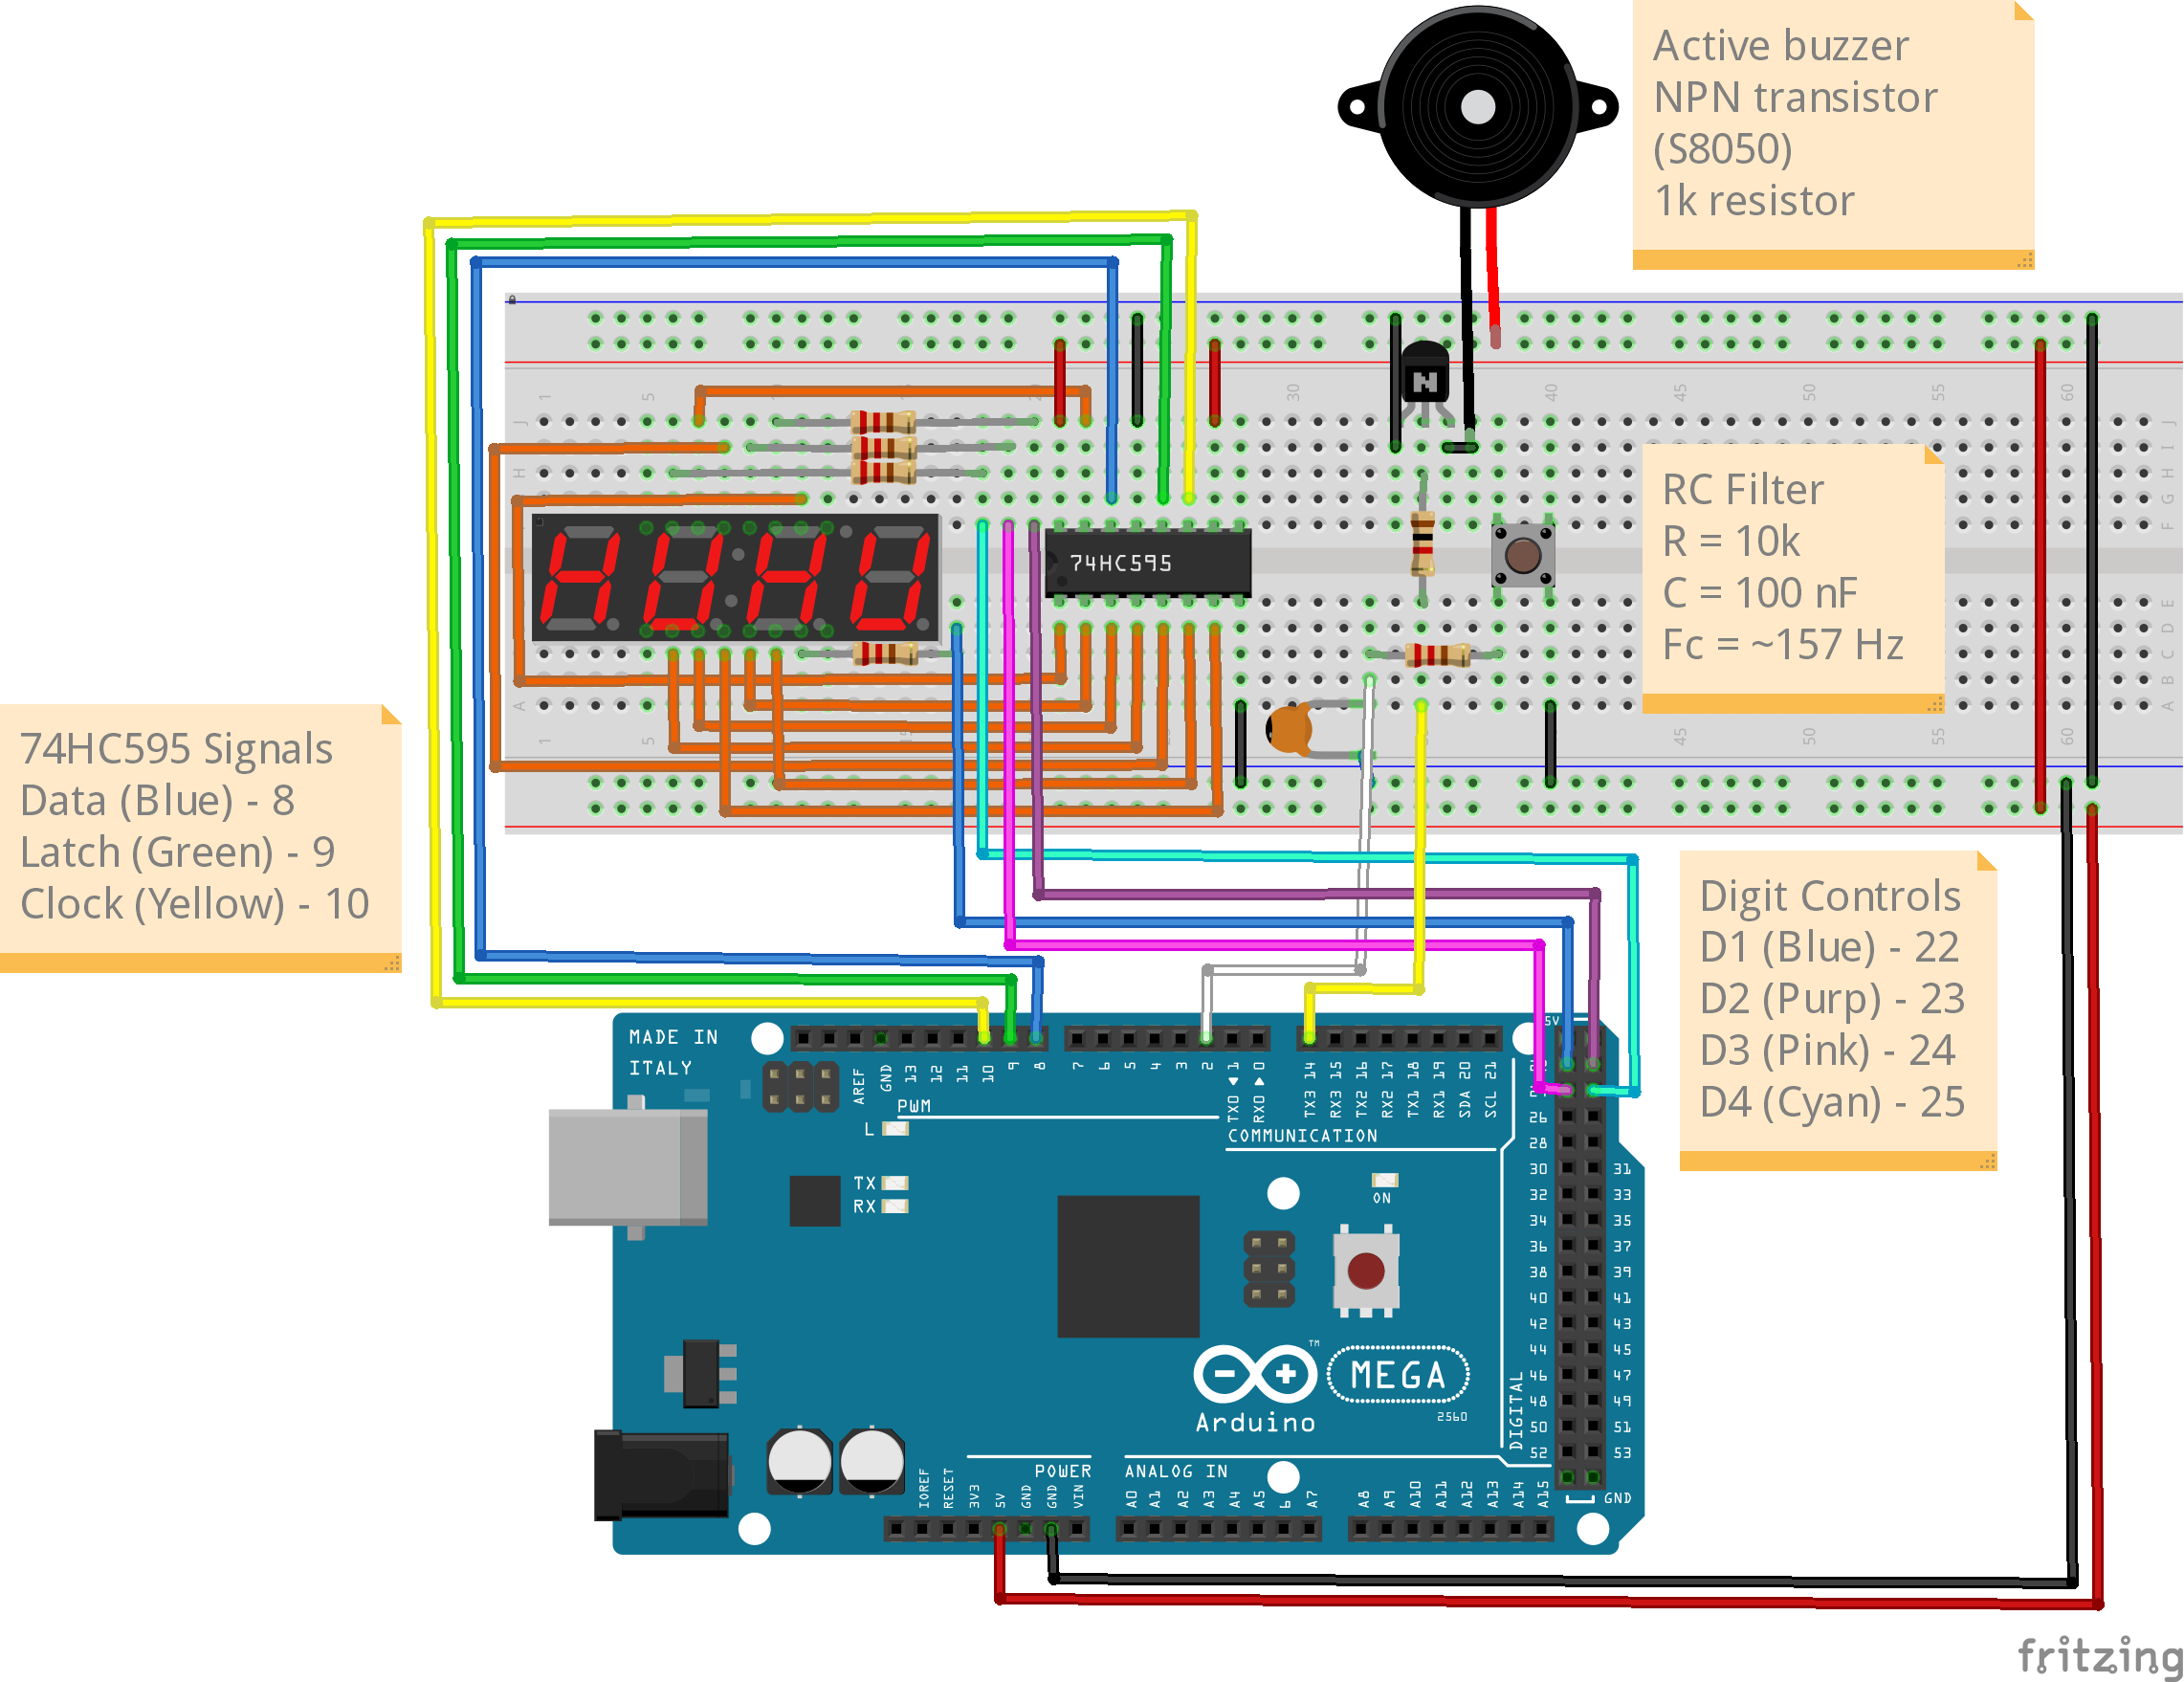
\includegraphics[]{p3_7seg_counter_ugrad_bb.png}
            \caption{The breadboard layout for Project 3}
            \label{fig:p3_7seg_counter_bb}
        \end{figure*}

        \subsubsection*{Arduino Code}
        Students should have a well-written and thought out program for this project.
        They should start by declaring the inputs and output pins, a table of bytes that represent various 7-segment digits according to the shift register hookup (provided in the project handout), an array representing the display, and any other global variables they need for the button reset and the buzzer.
        Students should have an ISR that triggers whenever the reset button is pressed and initializes the hold timer as well as flips a \lstinline[language=C++, style=mystyle]{BUTTON_PRESSED} flag.
        There should be a global variable tracking a current counter value that is counting something based on the \lstinline[language=C++, style=mystyle]{millis()} function (e.g. milliseconds/seconds/minutes since program start).

        In the \lstinline[language=C++, style=mystyle]{setup()} function, students should initialize their pins appropriately and attach the button ISR to the input pin depending on its configuration.
        For example, if the button is in an active HIGH configuration, the trigger would be the RISING edge; if it is active LOW, then the trigger would be the FALLING edge.

        For the \lstinline[language=C++, style=mystyle]{loop()} function, students should be checking if a pre-determined amount of time has passed between update calls (e.g. one millisecond/second/minute) and if it has, execute an update function that will update the display with the appropriate count.
        At the same time, they must reset the interval counter used to check the timing criteria.
        They should also be checking if a buzzer flag is active and if it is, sound the buzzer for a pre-determined amount of time.

        Students should have multiple other functions in this code to make it easier to follow. 
        For instance, the \lstinline[language=C++, style=mystyle]{updateCount()} function in the solution code takes the current count value and forms it into an array that can be displayed on the four display digits. They may also have functions that reset the display or perform other functions.

        \pagebreak
        \lstinputlisting[language=C++, style=mystyle]{../../../src/projects/project_3_7seg_counter_ugrad/project_3_7seg_counter_ugrad.ino}

\pagebreak
\section*{Graduate Students}
    \subsection*{Overview}
    For the graduate students, this project is meant to further expand upon the topics explored in Project 2 and apply them to a practical counter.
    Students will need to demonstrate incrementing a counter based on certain inputs such as "+5", "+10", +15", etc.
    The project will be considered successful when the following is demonstrated:
    
    \begin{enumerate}
        \item Buttons wired to appropriate inputs
            \begin{itemize}
                \item Three (3) of those buttons will determine how much the counter changes
                \item Two (2) of them will determine the counter's change in direction (either increment or decrement)
                \item The change buttons will be attached to digital interrupts to trigger the change in the counter
                \item Each press of the change buttons will sound a buzzer for auditory feedback
            \end{itemize}
        \item The current counter value will be displayed on a 4-digit, 7-segment display
        \item A schematic made in a "professional" manner (i.e. not Fritzing)
    \end{enumerate}

    \subsection*{Grading}
    \begin{tabular}{ | p{1in} | p{1.75in} | p{1.75in} | p{1.75in} | }
        \hline
        \textbf{Category} & \textbf{No Credit} & \textbf{Half Credit} & \textbf{Full Credit} \\

        \hline
        Efficacy (50 pts) & 
        Student did not demonstrate their working project & 
        student demonstrated a working project, but it did not meet all of the requirements specified in the project handout & 
        student demonstrated a feature-complete project that accomplished all of the goals specified in the project handout \\
        \hline
        Breadboard neatness (10 pts) & 
        Student did not show a breadboard, or it is exceptionally difficult to trace wires or diagnose &
        Student showed a breadboard, but it is difficult to trace or understand &
        Student showed a breadboard that is easy to follow and understand \\
        \hline
        Code neatness (20 pts) & 
        Student did not provide code, or it is difficult to read and follow &
        Student provided code, but it is difficult to read, variable names are nonsensical, functions are not documented or commented, code structure is not helpful &
        Student provided well-documented, easy to read and follow code pursuant to best coding practices and/or C++ standards \\
        \hline
        Schematic neatness (20 pts) & 
        Student did not provide a schematic, the schematic is of the Fritzing graphical type", or it is illegible &
        Student provided a schematic, but it is difficult to read or understand &
        Student provided a "professional-looking" schematic that is easy to read and understand \\
        \hline
        Extra credit (10 pts) &
        Student did not request extra credit or reach the necessary thresholds & 
        &
        Student successfully displayed a number larger than 9999 \\

        \hline
    \end{tabular}

        \subsubsection*{Extra Credit}
        The extra credit opportunity for this project is to count past 9999 on the 7-segment counter.
        This can be done in a variety of ways such as:
        
        \begin{itemize}
            \item Using a different base than decimal (e.g. hexadecimal)
            \item Using scientific notation (e.g. 10E4)
            \item A theater-chase (e.g. 10000 "sliding" across the display) \textit{WITH} a noticeable distinction between start and end of the sliding value
        \end{itemize}
\end{document}